\begin{frame}{Algorithm}
    \includegraphics[height=0.79\paperheight, keepaspectratio]{images/algo.png}    
\end{frame}

\begin{frame}{Algorithm}
\begin{itemize}
    \item Objective : to compute the nodes reachable from $\langle s_{main}, \mathbf{0} \rangle$ via interprocedurally valid paths in the exploded super graph $G^\#$.
    \item Worklist based algorithm
    \item Iteratively computes two sets : $\mathit{PathEdge}$ and $\mathit{SummaryEdge}$ using dynamic programming.
    \item The set $\mathit{PathEdge}$ stores special edges called \emph{path edges}. Every path edge begins at entry point of a procedure, and ends at some point in the procedure.
    \item First path edge added to the worklist: $\langle s_{main}, \mathbf{0} \rangle \rightarrow \langle s_{main}, \mathbf{0} \rangle$.
    \item In each iteration, a path edge $\langle s_p, d_1 \rangle \rightarrow \langle n, d_2 \rangle$ is removed from the worklist, and new path edge(s) and/or summary edge are added based on the type of $n$. (See Figures 3 and 4 in the paper)
\end{itemize}
\end{frame}

\begin{frame}{Cases}
    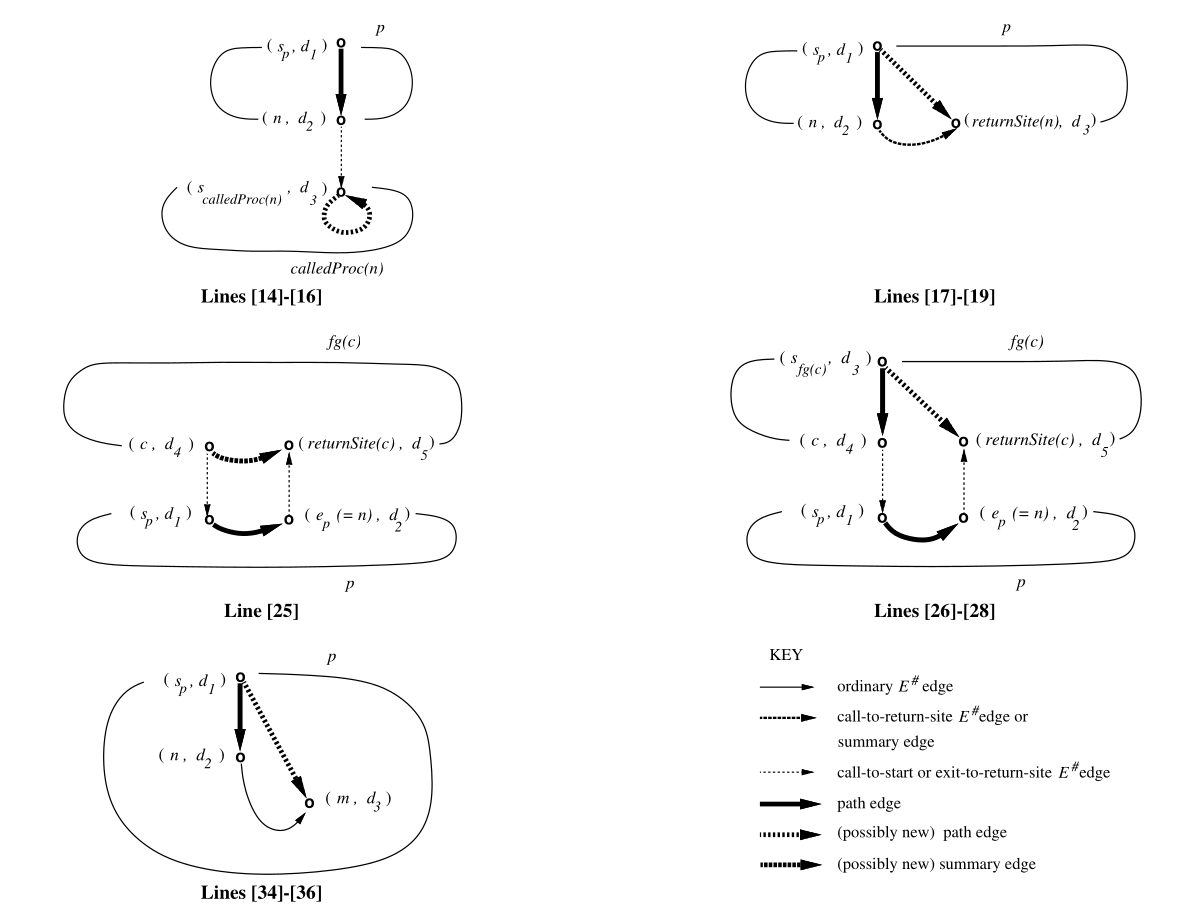
\includegraphics[height=0.79\paperheight, keepaspectratio]{images/tabulate.png}    
\end{frame}

\begin{frame}{Property of Path edges}
    \begin{itemize}
    \item Path edge $\langle s_{\text{\textit{procOf}}(N)}, d_1 \rangle \to \langle N, d_2 \rangle$ iff
    \begin{itemize}
        \item there is an inter-procedurally valid path from $\langle s_{\text{\textit{main}}}, \mathbf{0} \rangle$ to $\langle s_{\text{\textit{procOf}}(N)}, d_1 \rangle$, and
        \item there is an inter-procedurally valid and complete path from $\langle s_{\text{\textit{procOf}}(N)}, d_1 \rangle$ to $\langle N, d_2 \rangle$.
    \end{itemize}

    \item After the algorithm terminates, for any node $N$, the following set is equal to $\text{JVP}_N$:
    \begin{multline*}
    \{ d_2 \in D \mid \exists d_1 \in (D \cup \{\mathbf{0}\}) \text{ such that } \\
    (\langle s_{\text{\textit{procOf}}(N)}, d_1 \rangle, \langle N, d_2 \rangle) \in \text{\textit{PathEdge}} \}
    \end{multline*}
\end{itemize}
\end{frame}

\begin{frame}{Algorithm - $n$ is not a call or exit node}
\textbf{case} $n \in (N_p - Call_p - \{e_p\})$ :\\
\quad \textbf{for each} $\langle m, d_3 \rangle$ such that $\langle n, d_2 \rangle \to \langle m, d_3 \rangle \in E^\#$ \textbf{do}\\
\qquad $\text{Propagate}(\langle s_p, d_1 \rangle \to \langle m, d_3 \rangle)$\\
\quad \textbf{od}\\
\textbf{end case}
\vspace{0.5em}
\begin{center}    
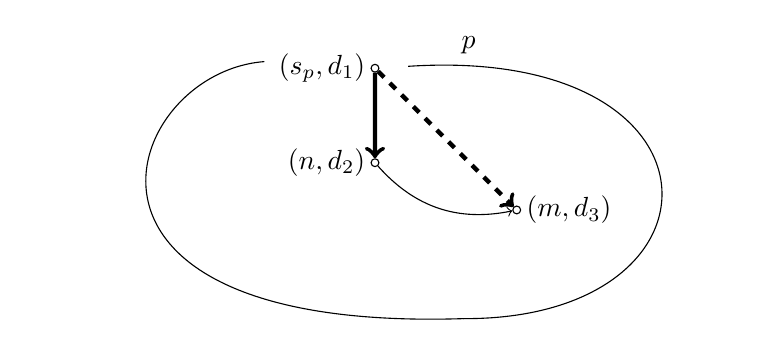
\begin{tikzpicture}[scale=1.2]
    \node at (0.49, 1.24) {$p$};

    \node[draw, circle, inner sep=1pt, fill=white] (sp) at (-0.5, 1) {};
    \node[left] (node1) at (sp) {$(s_p, d_1)$};

    \node[draw, circle, inner sep=1.pt, fill=white] (n) at (-0.5, 0) {};
    \node[left] at (n) {$(n, d_2)$};

    \node[draw, circle, inner sep=1pt, fill=white] (m) at (1, -0.5) {};
    \node[right] at (m) {$(m, d_3)$};

    \draw[->, ultra thick] (sp) -- (n);
    \draw[->] (n) to[bend right=30] (m);
    \draw[->, ultra thick, dashed] (sp) -- (m);
  \draw (-1.67,1.07) .. controls (-3.17,0.96) and (-4.17,-1.8) .. (0.44,-1.65);
  \draw (0.43,-1.65) .. controls (3.33,-1.67) and (3.33,1.25) .. (-0.15,1.02);
\end{tikzpicture}
\vspace{0.1em}
\text{Lines [34]-[36]}
\end{center}
\end{frame}

\begin{frame}{Algorithm - $n$ is a call node}
\begin{footnotesize}
\textbf{case} $n \in \mathit{Call}_p$ :\\
\quad \textbf{for each} $d_3$ such that $\langle n, d_2 \rangle \to \langle s_{\mathit{calledProc}(n)}, d_3 \rangle \in E^\#$ \textbf{do}\\
\qquad $\text{Propagate}(\langle s_{\mathit{calledProc}(n)}, d_3 \rangle \to \langle s_{\mathit{calledProc}(n)}, d_3 \rangle)$\\
\quad \textbf{od}\\
\quad \textbf{for each} $d_3$ such that $\langle n, d_2 \rangle \to \langle \mathit{returnSite}(n), d_3 \rangle \in (E^\# \cup \mathit{SummaryEdge})$ \textbf{do}\\
\qquad $\text{Propagate}(\langle s_p, d_1 \rangle \to \langle \mathit{returnSite}(n), d_3 \rangle)$\\
\quad \textbf{od}\\
\textbf{end case}
\end{footnotesize}
\end{frame}

\begin{frame}{Algorithm - $n$ is a call node}
\begin{center}
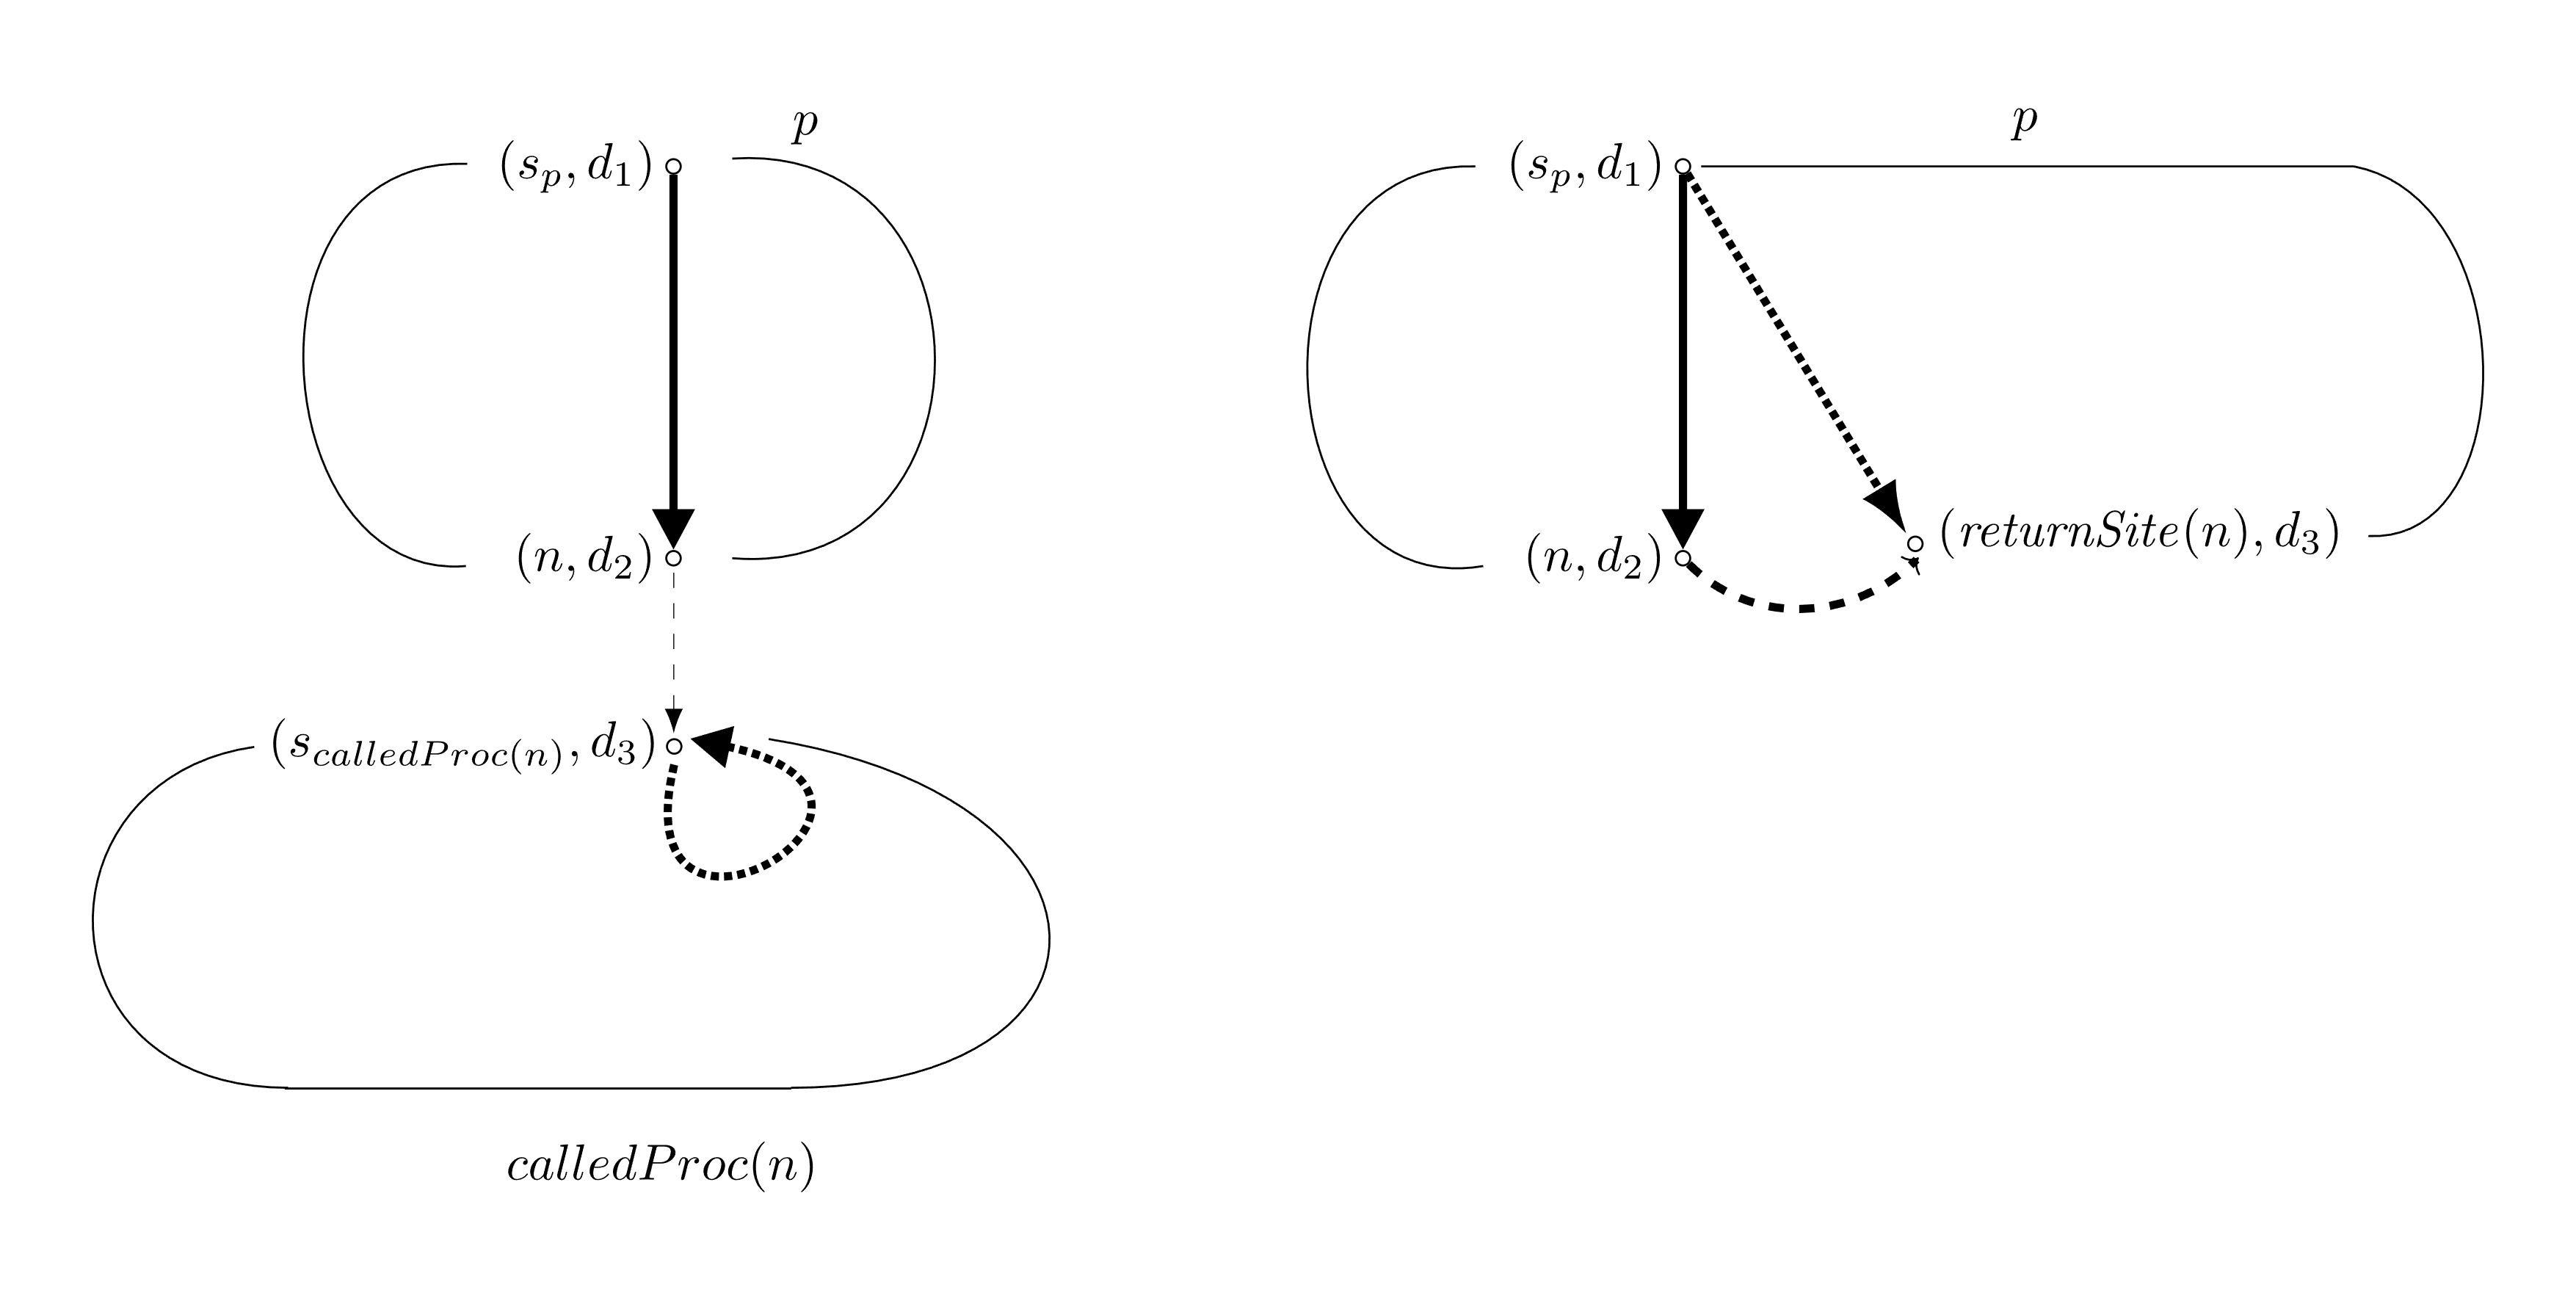
\includegraphics[width=0.9\textwidth]{images/tikz-export.png}
    \text{Lines [14]-[16]} \hspace{8em} \text{Lines [17]-[19]}
\end{center}
\end{frame}

\begin{frame}{Algorithm: Exit Nodes}
\begin{block}{Case \(n = e_p\)}
\textbf{For each} \(c \in \text{callers}(p)\):\\
\quad \textbf{For each} \(d_4, d_5\) such that
\(\langle c, d_4 \rangle \to \langle s_p, d_1 \rangle \in E^\#\) \textbf{and}
\(\langle e_p, d_2 \rangle \to \langle \text{returnSite}(c), d_5 \rangle \in E^\#\):\\
\quad\quad \textbf{if} \(\langle c, d_4 \rangle \to \langle \text{returnSite}(c), d_5 \rangle \notin \text{SummaryEdge}\):\\
\quad\quad\quad Insert into \text{SummaryEdge};\\
\quad\quad\quad \textbf{For each} \(d_3\) such that
\(\langle s_{\text{procOf}(c)}, d_3 \rangle \to \langle c, d_4 \rangle \in \text{PathEdge}\):\\
\quad\quad\quad\quad \(\text{Propagate}\bigl(\langle s_{\text{procOf}(c)}, d_3 \rangle \to \langle \text{returnSite}(c), d_5 \rangle\bigr)\)
\end{block}
\end{frame}

\begin{frame}{Algorithm Correctness}
    \begin{theorem}[4.1]
    Let $ X_N = \{ d_2 \in D \mid \exists d_1 \in (D \cup \{\mathbf{0}\}) \text{ such that } (\langle s_{\text{\textit{procOf}}(N)}, d_1 \rangle, \langle N, d_2 \rangle) \in \text{\textit{PathEdge}} \} $
    for the node $N$ after the algorithm terminates.
    
    Then $X_N = \text{JVP}_N$.
    \end{theorem}
\end{frame}

\begin{frame}{Proof of Theorem 4.1: First direction}
    \begin{itemize}
    \item Given: $\exists d_1 \in D \cup \{\mathbf{0}\}$ such that $(\langle s_{\text{\textit{procOf}}(N)}, d_1 \rangle, \langle N, d_2 \rangle) \in \text{\textit{PathEdge}}$ when the tabulation algorithm terminates.
    
    \item Invoking Theorem 3.8, it suffices to show that there is an inter-procedurally valid path in the exploded super graph from $\langle s_{\text{\textit{main}}}, \mathbf{0} \rangle$ to $\langle N, d_2 \rangle$.
    
    \item Argument is by induction on the number iterations of the main loop in the algorithm.
    
    \item Induction hypothesis:
    $\forall N, d_1, d_2, (\langle s_{\text{\textit{procOf}}(N)}, d_1 \rangle, \langle N, d_2 \rangle) \in \text{\textit{PathEdge}} \implies$
    \begin{itemize}
        \item there is an inter-procedurally valid path from $\langle s_{\text{\textit{main}}}, \mathbf{0} \rangle$ to $\langle s_{\text{\textit{procOf}}(N)}, d_1 \rangle$, and
        \item there is an inter-procedurally valid and complete path from $\langle s_{\text{\textit{procOf}}(N)}, d_1 \rangle$ to $\langle N, d_2 \rangle$.
    \end{itemize}
\end{itemize}
\end{frame}

\begin{frame}{Proof of Theorem 4.1: Other direction}
    \begin{itemize}
    \item Given there is an interprocedurally valid path from $\langle s_{\text{\textit{main}}}, \mathbf{0} \rangle$ to $\langle N, d_2 \rangle$
    
    \item To show that there exists $d_1 \in (D \cup \{\mathbf{0}\})$ such that $(\langle s_{\text{\textit{procOf}}(N)}, d_1 \rangle, \langle N, d_2 \rangle) \in \text{\textit{PathEdge}}$ when the tabulation algorithm terminates.
    \item Induction on the length of the path
    \item Induction hypothesis: $\forall N, d_2$, if there is an interprocedurally valid path of length $j$ from $\langle s_{\text{\textit{main}}}, \mathbf{0} \rangle$ to $\langle N, d_2 \rangle$, then there exists $(\langle s_{\text{\textit{procOf}}(N)}, d_1 \rangle, \langle N, d_2 \rangle) \in \text{\textit{PathEdge}}$ when the tabulation algorithm terminates.
\end{itemize}
\end{frame}

\begin{frame}{Efficiency}
    Complexity
\begin{itemize}
    \item $O(ED^3)$ for general IDFS problems
    \item $O(ED)$ for gen-kill problems (a special class of problems that includes available expressions, reaching definitions and live variables); comparable to best known algorithm specialized for gen-kill problems.
\end{itemize}

How it compares to iterative approach
\begin{itemize}
    \item Plain iterative would need time proportional to $|L|$, which is $2^{|D|}$.
    \item It's possible to produce a variant of iterative approach that works with values from $D$, instead of values from $L$. Still, its complexity is likely to be worse than $O(ED^3)$.
\end{itemize}
\end{frame}